\chapter{Commissioning of the AHCAL technological prototype}

Before every testbeam, all the electronics of the detector must be characterized. Before the full assembly, each individual chips must be tested in order to reject chips that presents bad channels or any other defects. After the assembly, each board needs to be characterized. This included the measurement of the SiPM-tile gain, the trigger threshold and noise. In this chapter, the testing of the chips and the commissioning procedure of the AHCAL will be presented.

\section{Testing of individual SPIROC2B chips}

The testing of individual chips prior to the soldering to the HBU board is necessarity. This avoids broken chips to be installed and reduces the number of dead channels. So far, the testing had to be done manually for each chip. This reduces the number of cross-checks done on the chips due to time constrains. The SPIROC2B chip can be tested standalone on a custom made PCB board. The SPIROC2B chip is installed in a special socket and is readout out by an ALTERA FPGA. The board is operated by a Labview software made by the OMEGA group \cite{}.

\begin{figure}[htbp!]
  \centering
  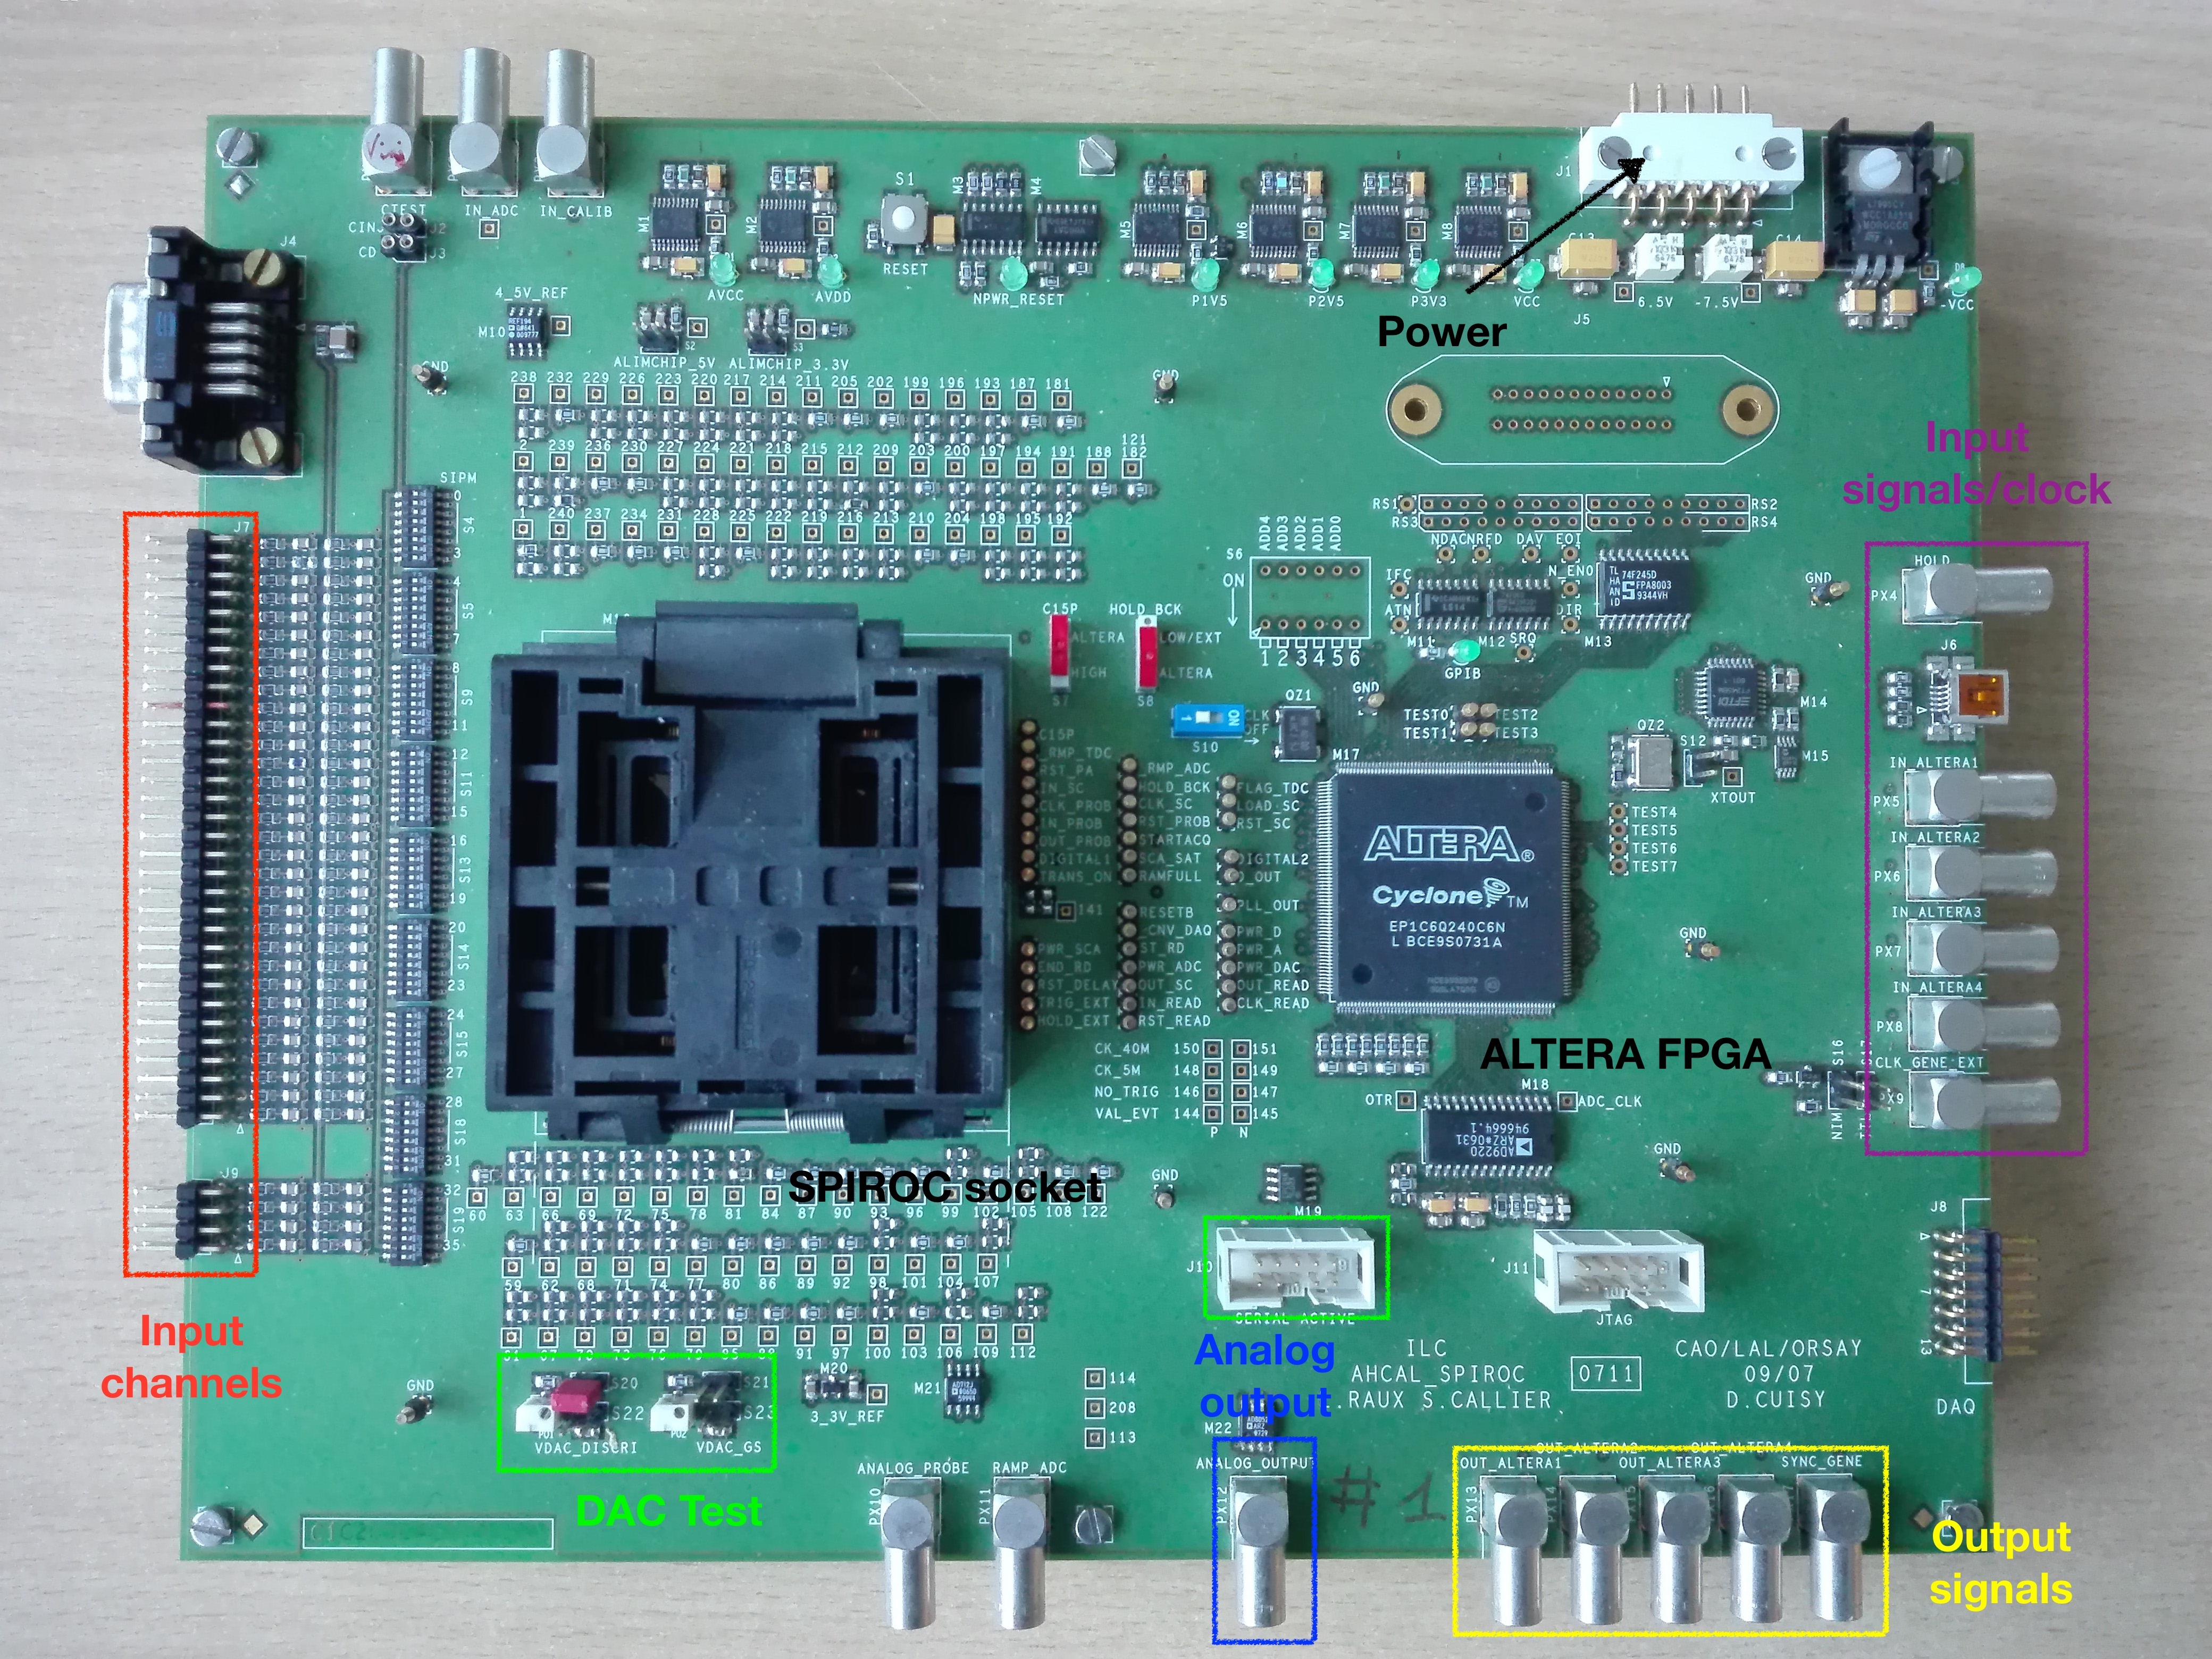
\includegraphics[width=1\linewidth]{chap4/fig_Commi/TestBoard.jpg}
  \caption{Testboard used to test the SPIROC2B chip standalone.} \label{fig:Testboard_SP2B}
\end{figure}

The board as shown in figure \ref{fig:Testboard_SP2B} contains all the debugging feature needed to check the functionning of the chip.

\section{Commissioning procedure}

\section{Noise Measurement in the AHCAL}
